\documentclass[conference]{IEEEtran}
\IEEEoverridecommandlockouts
\usepackage{cite}
\usepackage{amsmath,amssymb,amsfonts}
\usepackage{algorithmic}
\usepackage{graphicx}
\usepackage{textcomp}
\usepackage{xcolor}
\usepackage{booktabs}
\usepackage{url}
\usepackage{array}

\begin{document}

\title{AegisTag: Decentralized, Offline-Resilient Emergency Medical Information System using Web NFC and Zero-Trust Verification}

% CAMERA-READY: replace with the real author names, affiliations and e-mails.
\author{\IEEEauthorblockN{[Author names]}
\IEEEauthorblockA{[Affiliation, city, country] \\
{[e-mail addresses]}}
}

\maketitle

\begin{abstract}
Emergency care often needs a patient's allergies, blood group and DNR status exactly where networks fail. AegisTag stores a signed triage profile on a passive NFC wearable and verifies it entirely offline with a two-tier ECDSA scheme: a per-issuance tag key signs the patient ID, issue time and triage data, and a Healthcare Authority certificate binds that key to the same patient and issuance. A naive JSON/base64/gzip encoding exceeds the 504-byte NTAG215 budget by up to 208 bytes, whereas the compact binary encoding now deployed fits every realistic profile with 90--292 bytes to spare. On an Android phone, both verification tiers together take 0.51\,ms and the complete legacy scan path including decompression 2.09\,ms, about 1/650 of the 1.37\,s tap-to-render time. Across 2{,}600 adversarial trials in twelve attack classes, including relabelled, re-dated, superseded and revoked tags, no attack was accepted and no valid control was rejected; validly signed but stale tags are rejected only by a server-side freshness check, showing that signature validity alone does not establish currency. We also analyse cloning, revocation, authority-key compromise and unauthorized issuance, and release an in-browser NFC trial suite and all data for reproduction.
\end{abstract}

\begin{IEEEkeywords}
NFC, Emergency Medical System, Offline Resilience, Role-Based Access Control, Cryptographic Verification
\end{IEEEkeywords}

\section{Introduction}
\label{sec:intro}

\subsection{Emergency Medical Information Access Problem}
In emergency medical services (EMS), the first hour after a traumatic injury -- the ``golden hour'' -- is critical to outcomes, and the first ten minutes (the ``platinum ten minutes'') are considered decisive for life-threatening interventions. Responders must administer medications, intubate or transfuse without the patient's basic background (severe drug allergies, blood group, Do Not Resuscitate (DNR) directives), risking adverse drug events or contraindicated treatment.

\subsection{Problem With Current Solutions}
Electronic Health Record (EHR) systems depend on centralized cloud services and connectivity that is unavailable in disaster areas, remote zones, or congested networks. Medical jewelry and printed cards work offline but offer no tamper protection and cannot be updated without replacing the hardware.

\subsection{Why NFC?}
Near Field Communication (13.56\,MHz) lets passive, battery-less tags such as the NTAG21x family transmit data to a smartphone with a low cognitive-load ``tap'' and no proprietary reader hardware.

\subsection{Contributions}
\begin{itemize}
\item A signed, offline-verifiable triage tag format whose compact binary encoding is deployed and fits passive-tag memory, with a reproducible byte-cost comparison of four encodings (Section~\ref{sec:results}).
\item A two-tier ECDSA P-256 scheme with per-issuance keys and patient- and time-bound certificates, plus a server-side freshness and revocation check, validated against 2{,}600 adversarial trials.
\item A threat analysis covering tampering, stale-record replay, revocation, cloning, authority-key compromise and unauthorized issuance (Section~\ref{sec:threats}).
\item A consent-gated model for physician access to full records, opened only by a current, authority-certified scan of that patient's tag.
\item An open benchmarking methodology: payload size, mobile and server compute latency, tamper detection, and an in-browser multi-condition NFC trial suite, with all scripts and raw data released.
\end{itemize}

\section{Related Work}
\label{sec:related}

\subsection{NFC-Based Healthcare Systems}
Prior NFC healthcare deployments mostly use tags as index keys into a networked record: ward-round identification \cite{kostinger2013}, cloud-backed health cards \cite{ukalkar2017}, hospital medication safety \cite{lahtela2008}, an emergency-department NFC/EMR simulation \cite{jung2018}, and mHealth tracking \cite{ebere2022} all resolve the tag against a central database, and stop working when the network does.

\subsection{Emergency Medical Information Systems}
QR wristbands are clonable and wear-sensitive; USB-based personal health records \cite{marupally2009} expose the responder's device to malware; SMS queries need the connectivity this class of system exists to avoid.

\subsection{Security and Privacy in NFC Systems}
The NDEF Signature Record Type has documented record-composition and denial-of-service weaknesses \cite{roland2011}. Saeed and Walter authenticate tags offline with a challenge-response PKI and a dedicated Tag Authentication Record \cite{saeed2012}; AegisTag needs only a standard NDEF record \cite{ndef_spec}, at the cost of application-level signatures. ECC outperforms RSA by an order of magnitude on constrained CPUs \cite{gura2004}, consistent with the sub-millisecond verification we measure (Table~\ref{tab:latency}).

\subsection{Chip-Level Attestation vs.\ Content Authorship}
NTAG21x chips carry a factory \emph{originality signature} over the chip UID \cite{nxp_ntag_datasheet}. It proves the silicon is genuine but says nothing about who wrote the data or whether it was altered. AegisTag's signatures address the complementary threat: they bind the \emph{content} to an authority-certified issuance.

\subsection{Consent and Access Governance in EHR Systems}
Role-based access control dominates health information systems but is strained by modern authorization needs \cite{decarvalho2018}. Break-glass extensions grant audited emergency access \cite{brucker2009}, including for healthcare IoT \cite{yang2018}. AegisTag's consent gate is an instance of this pattern that is opened only by a verified, current, patient-bound scan event, not merely logged.

\subsection{Signed Health Credentials}
The closest deployed precedents are offline-verifiable vaccination credentials. SMART Health Cards carry an ES256-signed JWS over a DEFLATE-compressed FHIR bundle in a QR code, with issuer keys published as JWK sets and per-card revocation lists \cite{shc_spec}. The EU Digital COVID Certificate signs a CBOR/COSE token (ES256 or PS256) encoded in a QR code, under a public-key trust framework with revocation lists \cite{eu_dcc}. Both show that issuer-signed health data can be verified offline at scale. AegisTag differs in three respects: it targets passive NFC memory rather than a visual code, which is what makes encoding size decisive (Section~\ref{sec:results}); it uses a fresh key per issuance with a certificate bound to patient and issue time, so re-issuance supersedes old tags without distributing revocation lists; and the signed tag also gates a clinician's access to the full record (Section~\ref{sec:architecture}). Table~\ref{tab:compare} summarizes the comparison.

\begin{table}[htbp]
\caption{Comparison With Existing Approaches}
\begin{center}
\footnotesize
\setlength{\tabcolsep}{3pt}
\begin{tabular}{lcccc}
\toprule
 & \textbf{ID-only} & \textbf{Signed QR} & \textbf{Medical} & \textbf{Aegis-} \\
\textbf{Property} & \textbf{NFC} & \textbf{credential} & \textbf{ID / card} & \textbf{Tag} \\
\midrule
Data available offline & -- & \checkmark & \checkmark & \checkmark \\
Tamper evident & -- & \checkmark & -- & \checkmark \\
Issuer authenticity & -- & \checkmark & -- & \checkmark \\
Supersession / revocation & n/a & lists & -- & \checkmark \\
Gates full-record access & -- & -- & -- & \checkmark \\
Updatable in place & \checkmark & \checkmark & -- & \checkmark \\
Read in a browser, no app & -- & -- & n/a & \checkmark$^\ast$ \\
\bottomrule
\multicolumn{5}{l}{\scriptsize ID-only NFC: \cite{kostinger2013,ukalkar2017,lahtela2008,jung2018,ebere2022}; signed QR: \cite{shc_spec,eu_dcc}.} \\
\multicolumn{5}{l}{\scriptsize $^\ast$Chromium on Android only (Section~\ref{sec:platform}).}
\end{tabular}
\label{tab:compare}
\end{center}
\end{table}

\subsection{Research Gap}
No prior system combines offline data availability, decentralized verification within passive-tag memory, freshness and revocation for long-lived offline tokens, \emph{and} a governed policy for elevating a clinician to full record access, backed by reproducible measurements.

\section{System Requirements and Threat Model}
\label{sec:requirements}

\subsection{Functional Requirements}
\begin{enumerate}
\item \textit{Offline Access}: render name, blood group, allergies, DNR status and emergency contacts with no network.
\item \textit{Integrity and Authenticity}: verify that the content was issued under a Healthcare Authority certificate and not altered since.
\item \textit{Currency}: when online, recognize a validly signed tag that has been superseded or revoked.
\item \textit{Web-Native Access}: scan from a browser without installing an app.
\item \textit{Governed Deep Access}: restrict full histories to a patient's primary physician or a clinician with a recent, current, certified scan.
\end{enumerate}

\subsection{Adversary Model}
An adversary may hold, read, rewrite or copy a patient's tag; replay an old but genuine tag; write tags of their own; obtain a clinician account; or, in the worst case, steal the authority signing key. A separate insider threat is a valid clinician browsing histories of patients they neither treat nor scanned. Eavesdropping is limited by keeping only non-stigmatizing triage data on the tag. Section~\ref{sec:threats} maps each threat to its mechanism and evidence.

\section{AegisTag Architecture and Implementation}
\label{sec:architecture}

\subsection{High-Level Architecture}
Fig.~\ref{fig:architecture} shows the four components. The \textit{Tag Writer} runs in the browser of a logged-in doctor whose account the Healthcare Authority has verified; self-registered clinician accounts gain no clinical access until verified, and there is no shared password. The \textit{passive NFC wearable} holds the signed record. The \textit{Responder/Doctor Client} reads and verifies tags with Web NFC \cite{w3c_webnfc} and Web Crypto, and renders the profile on-device. The \textit{Backend API} (Node.js/Express, PostgreSQL via Prisma) holds the authority signing key, issues certificates, records issuance and scans, and mediates access to full histories.

\begin{figure}[htbp]
\centering
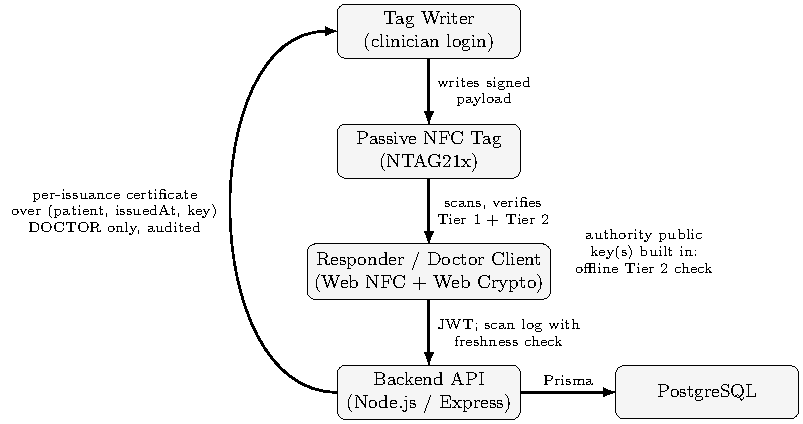
\includegraphics[width=\linewidth]{../paper/figures/architecture.pdf}
\caption{AegisTag architecture. The authority private key never leaves the backend; its public key is built into the client for offline Tier~2 verification.}
\label{fig:architecture}
\end{figure}

\subsection{NFC Data Layer}
Tags are written in the compact V3 encoding (Section~\ref{sec:results}): one NDEF record of TNF \emph{Unknown} carrying a length-prefixed binary layout with the SEC1-compressed tag key and raw 64-byte signatures. The reader also accepts the legacy V1 encoding (gzip-compressed JSON in a text record) and \emph{ID-only} tags that carry just the account number for online lookup, which fit even 144-byte NTAG213 chips but provide no offline data. The deployed hardware is NTAG216 (888~B); the 504-byte NTAG215 budget is used as a portability stress test.

\subsection{Access Control and Consent}
Roles (Patient, Doctor, First Responder) are assigned server-side at login and embedded in a signed JWT; no authorization decision uses a client-supplied role. A doctor may read a patient's full history only if they are the recorded primary physician or have a \emph{certified} scan of that patient within 24\,hours. A scan is logged only after the server re-verifies the raw tag, checks that the tag's \emph{signed} patient ID equals the requested account, and classifies its freshness. It is marked certified, a server-computed column and the only input the consent gate reads, only for an authority-certified tag that is the patient's current issuance.

\subsection{Implementation}
The backend is Node.js/TypeScript with Zod validation and bcrypt. The client is a React/Vite/TypeScript application using Web NFC and Web Crypto. All NFC access goes through one module that allows a single pending operation, applies timeouts, handles unreadable tags via the \texttt{readingerror} event, retries only transient I/O errors, and keeps the screen awake during an operation.

\section{Security Design}
\label{sec:security}

\subsection{Two-Tier Offline Verification}
For each issuance the Tag Writer generates a fresh, non-extractable ECDSA P-256 key pair \cite{johnson2001}. \textit{Tier~1}: the tag key signs a domain-separated, canonical encoding of the format version, patient ID, issue time and triage data. \textit{Tier~2}: the backend signs a separate domain-separated message binding (patient ID, issue time, tag public key) with the authority key. It does so only for an authenticated DOCTOR and records the issuing clinician and issue time. The private tag key is discarded after signing, so no long-lived key remains on staff devices. A reader verifies both tiers against the built-in authority key list without network access. Both tiers use raw IEEE~P1363 signatures, verified identically by Node.js and Web Crypto.

\subsection{Freshness and Revocation}
Re-issuing a patient's tag records a new issue time and thereby supersedes all earlier tags; a patient can also revoke every tag issued so far (e.g., when lost). Online, the server classifies each scanned tag as current, superseded, revoked or unregistered, and only a current tag can be certified. All verified scans are still logged, and superseded, revoked or unregistered-but-certified tags return an alert to the clinician. Offline, a reader cannot learn of revocation; it shows the issue date and flags tags older than one year.

\subsection{Keys and Sessions}
The authority private key exists only in server configuration, and the server derives its own trust anchor from it, so server and client cannot silently disagree. Clients accept a list of authority public keys to allow rotation. Refresh tokens live in an HTTP-only, \texttt{SameSite=Strict} cookie scoped to the authentication path, and access tokens are held in memory only, so script injection cannot read either from storage.

\subsection{Threat Analysis}
\label{sec:threats}
Table~\ref{tab:threats} maps the threats raised in review to mechanisms and evidence.

\begin{table}[htbp]
\caption{Threats, Mechanisms and Evidence}
\begin{center}
\footnotesize
\begin{tabular}{>{\raggedright\arraybackslash}p{1.65cm}>{\raggedright\arraybackslash}p{3.65cm}>{\raggedright\arraybackslash}p{1.7cm}}
\toprule
\textbf{Threat} & \textbf{Mechanism} & \textbf{Evidence} \\
\midrule
Tampering, forgery & Tier~1 over ID, time, data; Tier~2 binds key to ID and time & 9 tamper classes, 0/1{,}800 accepted \\
Stale replay & Signed issue time; server freshness check & superseded class, 0/200 \\
Lost/stolen tag & Patient revocation; alert on scan & revoked class, 0/200 \\
Relabelling to unlock records & Signed ID must match account & relabel and cert-graft classes \\
Cloning & A verbatim clone carries authentic data; consent window limited to that patient, current tag, logged & not prevented (Sec.~\ref{sec:limitations}) \\
Unauthorized issuance & Certificates only for Authority-verified, audited doctor accounts; fresh key per tag & server tests \\
Authority-key compromise & Key list rotation; online, certificates matching no recorded issuance raise an alert & offline readers trust it until updated \\
\bottomrule
\end{tabular}
\label{tab:threats}
\end{center}
\end{table}

\textit{Proposition (certified-scan unforgeability).} Assume ECDSA P-256 is existentially unforgeable under chosen-message attack (EUF-CMA), the authority key is secret, and the issuance service signs only after verifying the requesting doctor. Then an adversary without the authority key cannot make the server accept, as certified and current for patient $P$, any tag other than a copy of the one issued for $P$'s latest issue time $t$.

\textit{Proof sketch.} Acceptance requires a valid authority signature on the domain-separated message $(\textsf{cert}, P, t, pk)$ and $t$ equal to $P$'s recorded issuance. The authority signs exactly one such message per recorded $(P, t)$, with the $pk$ generated by the issuing client, so any other $pk$, $P$ or $t$ would be an authority forgery. With that $pk$, the content must carry a valid signature under its private key on $(\textsf{content}, v, P, t, d)$. That key signed exactly one message and was then discarded, so any different content $d$ would be a forgery under $pk$. Domain separation stops either signature from being reused as the other. Hence the only accepted tags are byte-equivalent copies of the genuine current tag, the cloning case discussed in Section~\ref{sec:limitations}. \hfill$\square$

\subsection{Platform Reach}
\label{sec:platform}
Web NFC is available only in Chromium on Android; iOS Safari has none. iOS can read NDEF tags through Core NFC in native apps, and because V3 is a standard NDEF record verified with standard ECDSA, a native iOS reader could reuse the same canonical encoding; we have not built or evaluated one. iOS users therefore depend on ID-only online lookup or a companion Android device today.

\section{Results and Discussion}
\label{sec:results}

\subsection{Methodology}
We measure payload size across four encodings and a profile-size sweep; compute latency on a real Android phone and a Node.js reference; tamper detection across twelve attack classes plus a control; and physical NFC reliability. All scripts, raw results and the generators for every table and figure are public\footnote{\url{https://github.com/nh-44/lifetag}; every table and figure is regenerated from \texttt{results/*.json} by \texttt{bench/generate-tables.ts} and \texttt{bench/plot\_*.py}.}; no number is hand-typed.

\subsection{Payload Encoding Comparison}
Table~\ref{tab:encoding} compares four encodings of the Medium profile against the 504-byte NTAG215 stress budget. The legacy encoding (V1: JWK key, base64 signatures, gzip) exceeds it by 68~bytes, and by 208~bytes for the Large profile; changing only the compressor (V2) does not close the gap. V3 stores a SEC1-compressed point and raw P1363 signatures in a binary record, removing the JSON/base64 overhead and the $\sim$33\% base64 tax, and fits with 230~bytes to spare (Fig.~\ref{fig:payload}). DEFLATE on top of V3 (V4) is marginally \emph{larger}, because keys and signatures leave little redundancy. V3 is the encoding the Tag Writer now uses by default; its client implementation reproduces the benchmark's byte counts exactly (274~B for the Medium profile).

\begin{figure}[htbp]
\centering
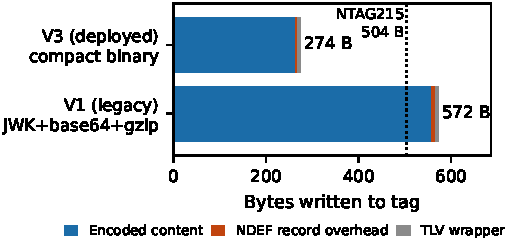
\includegraphics[width=\linewidth]{../paper/figures/payload_layout.pdf}
\caption{Bytes on tag, V1 vs.\ V3, Medium profile.}
\label{fig:payload}
\end{figure}

\begin{table}[htbp]
\caption{Payload Encoding Comparison, Medium Profile (measured)}
\begin{center}
\small
\resizebox{\ifdim\width>\columnwidth\columnwidth\else\width\fi}{!}{\begin{tabular}{lrrcr}
\toprule
\textbf{Variant} & \textbf{Content} & \textbf{On tag} & \textbf{Fits} & \textbf{Margin} \\
 & (B) & (B) & 504\,B & (B) \\
\midrule
V1 JSON/b64/gzip (legacy) & 557 & 572 & No & -68 \\
V2 JSON/b64/DEFLATE & 533 & 548 & No & -44 \\
V3 binary (deployed) & 263 & 274 & Yes & +230 \\
V4 binary/DEFLATE & 268 & 279 & Yes & +225 \\
\bottomrule
\end{tabular}}
\label{tab:encoding}
\end{center}
\end{table}


\subsection{Sensitivity to Profile Size}
Sweeping allergies (0--10) and contacts (1--3) with V3, every realistic combination fits the 504-byte budget with 90+ bytes to spare (Fig.~\ref{fig:sensitivity}); headroom runs out only at an unrealistic 20--25 allergies.

\begin{figure}[htbp]
\centering
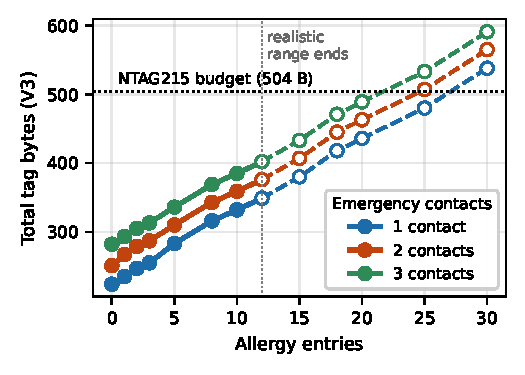
\includegraphics[width=\linewidth]{../paper/figures/sensitivity.pdf}
\caption{Total tag bytes (V3) vs.\ allergy count, by contact count. Dashed segments beyond 12 allergies reuse allergen names to locate the crossover and are not clinically realistic.}
\label{fig:sensitivity}
\end{figure}

\subsection{Compute Overhead}
Table~\ref{tab:latency} reports each operation on an Android phone (Chrome, n=100 after 20 warm-up runs) with a Node.js reference. Both verification tiers together take 0.51\,ms (0.25 + 0.26\,ms). The complete legacy V1 scan path, which adds gzip decompression, takes 2.09\,ms (p95 2.70\,ms), roughly 1/650 of the 1.37\,s tap-to-render time; V3 has no decompression step. Chrome limits the page timer to 0.1\,ms here, so sub-millisecond means are resolution-limited. Compute is not the bottleneck of a scan.

\begin{table}[htbp]
\caption{Cryptographic \& Compression Latency --- CPH2487, Android 10, Chrome 151.0.0.0 (n=100, 20 warm-up; mobile timer resolution 0.1\,ms). Node: server-class reference.}
\begin{center}
\small
\resizebox{\ifdim\width>\columnwidth\columnwidth\else\width\fi}{!}{\begin{tabular}{lrrrr}
\toprule
 & \multicolumn{3}{c}{\textbf{Mobile (ms)}} & \textbf{Node} \\
\textbf{Operation} & Mean & Median & p95 & Mean (ms) \\
\midrule
ECDSA Key Generation & 0.11 & 0.10 & 0.20 & 0.027 \\
Signature Creation & 0.14 & 0.10 & 0.20 & 0.020 \\
Tier 1 Verification & 0.25 & 0.30 & 0.30 & 0.051 \\
Tier 2 Verification & 0.26 & 0.30 & 0.30 & 0.053 \\
Gzip Compression & 1.27 & 1.20 & 1.70 & 0.020 \\
Gzip Decompression & 1.34 & 1.10 & 1.90 & 0.008 \\
Scan-Path Total & 2.09 & 2.00 & 2.70 & 0.117 \\
\bottomrule
\end{tabular}}
\label{tab:latency}
\end{center}
\end{table}


\subsection{Physical NFC Reliability}
\label{sec:nfc-results}
Initial single-condition trials on NTAG216 at about 1\,cm (Table~\ref{tab:nfc}) succeeded in 20/20 reads (1.37\,s mean tap-to-render) and 13/15 writes (86.7\%, Wilson 95\% CI 62--96\%), with the two failures returning \texttt{AbortError}. The timings run from the button press and so include moving the tag to the phone. Analysis of the write path traced the cancellations to a second write started while one was pending, which Chrome resolves by cancelling the first, and found that unreadable tags were never reported because the code listened for the wrong event. Both are fixed by the single-operation NFC module (Section~\ref{sec:architecture}), and writes now start in a dedicated user gesture after certification completes.

\begin{table}[htbp]
\caption{Initial Single-Condition NFC Trials, NTAG216, ~1\,cm coplanar bare tag (measured; times include moving the tag to the phone)}
\begin{center}
\small
\resizebox{\ifdim\width>\columnwidth\columnwidth\else\width\fi}{!}{\begin{tabular}{lrrrr}
\toprule
\textbf{Operation} & \textbf{N} & \textbf{Success} & \textbf{Mean (ms)} & \textbf{Median (ms)} \\
\midrule
Read (handshake) & 20 & 100\% & 1338 & 934 \\
Read (tap-to-render) & 20 & 100\% & 1368 & 967 \\
Write (handshake) & 15 & 86.7\% & 4294 & 2199 \\
\bottomrule
\end{tabular}}
\label{tab:nfc}
\end{center}
\end{table}


To answer how reliability varies with conditions, the client includes an NFC trial suite that runs every trial through the production NFC and codec code. It generates randomized full-factorial plans over distance (0--4\,cm), orientation (0--90$^\circ$), medium (bare, wristband, phone case, metal, skin), placement (tag approached vs.\ resting before start, separating hand movement from system latency), encoding (V1, V3) and payload size, and covers read, write, overwrite, overwrite-protection, erase and tampered-tag trials with read-back verification. Each result is reported with a Wilson interval.
\IfFileExists{../paper/tables/nfc-lab.tex}{Table~\ref{tab:nfclab} summarizes these trials by operation\IfFileExists{../paper/tables/nfc-lab-factors.tex}{ and Table~\ref{tab:nfcfactors} by condition}{}.
\input{../paper/tables/nfc-lab.tex}
\IfFileExists{../paper/tables/nfc-lab-factors.tex}{\input{../paper/tables/nfc-lab-factors.tex}}{}}{}

\subsection{Tamper Detection}
Table~\ref{tab:tamper} reports 2{,}600 trials. A trial counts as \emph{accepted} only if the tag is authority-certified \emph{and} the patient's current issuance, the exact condition for a certified scan. Self-signed tags legitimately pass Tier~1, so certification and currency, not internal consistency, are what must be unforgeable. No attack trial was accepted and no control was rejected. Re-dating an old tag or relabelling it for another patient breaks Tier~1; reusing a genuine certificate for another patient breaks Tier~2. Superseded and revoked tags carry \emph{fully valid} signatures (200/200 each) and are rejected only by the freshness check. Because acceptance would require an ECDSA forgery, these trials test the implementation against the proposition of Section~\ref{sec:threats} rather than estimate a probability; read statistically, 0 accepted out of 2{,}400 attack trials bounds the per-trial acceptance rate below 0.13\% at 95\% confidence.

\begin{table}[htbp]
\caption{Tamper Detection, 2600 Trials (measured). A trial is accepted only if the tag is authority-certified and the patient's current issuance.}
\begin{center}
\small
\resizebox{\ifdim\width>\columnwidth\columnwidth\else\width\fi}{!}{\begin{tabular}{lrrr}
\toprule
\textbf{Class} & \textbf{Accepted} & \textbf{Cert.\ valid} & \textbf{Anom.} \\
\midrule
Content corruption & 0/200 & 0/200 & 0 \\
Public key corruption & 0/200 & 0/200 & 0 \\
Patient sig.\ corruption & 0/200 & 0/200 & 0 \\
Authority sig.\ corruption & 0/200 & 0/200 & 0 \\
Random truncation & 0/200 & 0/200 & 0 \\
Cross-patient content graft & 0/200 & 0/200 & 0 \\
Forged key (Tier 2 attack) & 0/200 & 0/200 & 0 \\
issuedAt edit & 0/200 & 0/200 & 0 \\
Patient-ID relabel & 0/200 & 0/200 & 0 \\
Certificate graft & 0/200 & 0/200 & 0 \\
Superseded-tag replay$^\dagger$ & 0/200 & 200/200 & 0 \\
Revoked-tag replay$^\dagger$ & 0/200 & 200/200 & 0 \\
Valid current tag (control) & 200/200 & 200/200 & 0 \\
\bottomrule
\multicolumn{4}{l}{\footnotesize $^\dagger$Signatures valid; rejected only by the freshness check.}
\end{tabular}}
\label{tab:tamper}
\end{center}
\end{table}


\subsection{Cost of Trust}
Against an unsigned plaintext baseline with the same fields, the signed V1 payload costs +325~bytes on tag, while added compute is about 0.1\,ms on the server reference. The cost of trust is a byte-budget cost, which the V3 encoding removes.

\subsection{Discussion}
Two lessons generalize. First, encoding choice, not the presence of cryptography, decides whether a signed profile fits passive-tag memory: V1 and V3 carry identical guarantees but differ by 298~bytes. Second, the defects we found surfaced only under cross-boundary testing. The original evaluation found a DER-versus-P1363 signature mismatch and an empty-allergy normalization bug. Re-examining the threat model for this revision found that freshness metadata and patient identity were not signed, and that scans were not bound to the requested patient. The re-dating and relabelling attack classes now test these paths directly.

\textit{Data protection.} The tag holds only the minimum triage set; full histories stay on the server behind the consent gate. Every tag scan and online lookup is logged, and the patient can see who accessed their record and when, which supports the notice and accountability duties of India's Digital Personal Data Protection Act, 2023 \cite{dpdp2023}. Because the triage profile already maps to HL7 FHIR resources, issuance could be linked to a patient's ABHA identity under the Ayushman Bharat Digital Mission \cite{abdm}.

\section{Limitations and Future Work}
\label{sec:limitations}

\subsection{Limitations}
\begin{itemize}
\item The certificate binds a key to an issuance and the server records the issuing clinician, but the tag does not carry the clinician's signature, and no signature attests clinical accuracy.
\item Static NFC tags cannot answer challenges, so a byte-exact clone of a valid tag cannot be distinguished offline. It carries only authentic data, and online it opens the consent window only for that patient while the tag is current.
\item Offline readers cannot learn of revocation or supersession, and after an authority-key compromise they trust forged certificates until the client's key list is updated.
\item Web NFC is unavailable on iOS; the physical trials so far use one Android device and one NTAG216 tag type.
\end{itemize}

\subsection{Future Work}
Clinician co-signature on the tag; binding the chip UID or originality signature into the signed content to stop copies onto blank tags; a native iOS reader using Core NFC; a vetted post-quantum certification step; ABHA-linked issuance through ABDM; multi-site trials across devices and tag vendors.

\section{Conclusion}
AegisTag stores a signed triage profile on a passive NFC tag and verifies it offline with per-issuance keys and patient- and time-bound certificates, while a server-side freshness check and consent gate govern online use. Encoding choice alone removes the byte-budget risk, verification adds well under a millisecond against a one-second tap, and 2{,}600 adversarial trials, including stale and revoked tags, produced no false accept or reject. We release the code, data and an NFC trial suite so these results can be reproduced and extended.

\begin{thebibliography}{00}
\bibitem{kostinger2013} H. K\"ostinger, M. Gobber, T. Grechenig, B. Tappeiner, and W. Schramm, ``Developing a NFC based patient identification and ward round system for mobile devices using the android platform,'' in \textit{2013 IEEE Point-of-Care Healthcare Technologies (PHT)}, Bangalore, India, 2013, pp. 176--179.
\bibitem{ukalkar2017} G. V. Ukalkar and P. S. Halgaonkar, ``Cloud based NFC health card system,'' in \textit{2017 Int. Conf. on Intelligent Computing and Control Systems (ICICCS)}, 2017.
\bibitem{lahtela2008} A. Lahtela, M. Hassinen, and V. Jylh\"a, ``RFID and NFC in healthcare: Safety of hospitals medication care,'' in \textit{Proc. 2nd Int. ICST Conf. on Pervasive Computing Technologies for Healthcare (PervasiveHealth)}, 2008.
\bibitem{jung2018} K. Y. Jung, T. Kim, J. Jung, J. Lee, J. S. Choi, M. Kang, D. K. Chang, and W. C. Cha, ``The effectiveness of near-field communication integrated with a mobile electronic medical record system: emergency department simulation study,'' \textit{JMIR mHealth and uHealth}, vol. 6, no. 9, e185, 2018.
\bibitem{ebere2022} O. Ebere, V. Ramsurrun, P. Seeam, P. Katsina, S. Anantwar, M. Sharma, and A. Seeam, ``NFC tag-based mHealth patient healthcare tracking system,'' in \textit{2022 3rd Int. Conf. on Next Generation Computing Applications (NextComp)}, 2022.
\bibitem{marupally2009} P. R. Marupally, V. Paruchuri, and S. Chellappan, ``Privacy preserving portable health record (P\textsuperscript{3}HR),'' in \textit{Proc. 2009 12th Int. Conf. on Network-Based Information Systems (NBiS)}, 2009.
\bibitem{roland2011} M. Roland, J. Langer, and J. Scharinger, ``Security vulnerabilities of the NDEF signature record type,'' in \textit{Proc. 2011 3rd Int. Workshop on Near Field Communication (NFC)}, 2011, pp. 65--70.
\bibitem{saeed2012} M. Q. Saeed and C. D. Walter, ``Off-line NFC tag authentication,'' in \textit{Proc. 7th Int. Conf. for Internet Technology and Secured Transactions (ICITST-2012)}, 2012.
\bibitem{ndef_spec} NFC Forum, ``NFC Data Exchange Format (NDEF) Technical Specification.''
\bibitem{gura2004} N. Gura, A. Patel, A. Wander, H. Eberle, and S. C. Shantz, ``Comparing elliptic curve cryptography and RSA on 8-bit CPUs,'' in \textit{Cryptographic Hardware and Embedded Systems -- CHES 2004}, LNCS vol. 3156, Springer, 2004, pp. 119--132.
\bibitem{nxp_ntag_datasheet} NXP Semiconductors, ``NTAG213/215/216 NFC Forum Type 2 Tag compliant IC,'' Data sheet.
\bibitem{decarvalho2018} M. A. de Carvalho Junior and P. Bandiera-Paiva, ``Health information system role-based access control current security trends and challenges,'' \textit{Journal of Healthcare Engineering}, vol. 2018, pp. 1--8, 2018.
\bibitem{brucker2009} A. D. Brucker and H. Petritsch, ``Extending access control models with break-glass,'' in \textit{Proc. 14th ACM Symp. on Access Control Models and Technologies (SACMAT)}, Stresa, Italy, 2009, pp. 197--206.
\bibitem{yang2018} Y. Yang, X. Liu, and R. H. Deng, ``Lightweight break-glass access control system for healthcare Internet-of-Things,'' \textit{IEEE Transactions on Industrial Informatics}, vol. 14, no. 8, 2018.
\bibitem{shc_spec} Vaccination Credential Initiative, ``SMART Health Cards Framework,'' specification. [Online]. Available: \url{https://spec.smarthealth.cards/}
\bibitem{eu_dcc} European Commission, ``Commission Implementing Decision (EU) 2021/1073 of 28 June 2021 laying down technical specifications and rules for the implementation of the trust framework for the EU Digital COVID Certificate,'' \textit{Official Journal of the European Union}, 2021.
\bibitem{w3c_webnfc} W3C, ``Web NFC API,'' Editor's Draft, 2023.
\bibitem{johnson2001} D. Johnson, A. Menezes, and S. Vanstone, ``The Elliptic Curve Digital Signature Algorithm (ECDSA),'' \textit{International Journal of Information Security}, vol. 1, no. 1, pp. 36--63, 2001.
\bibitem{dpdp2023} Government of India, ``The Digital Personal Data Protection Act, 2023 (No. 22 of 2023),'' \textit{The Gazette of India}, Aug. 2023.
\bibitem{abdm} National Health Authority, Government of India, ``Ayushman Bharat Digital Mission (ABDM).'' [Online]. Available: \url{https://abdm.gov.in}
\end{thebibliography}

\end{document}
